In this Section we will cover what kind of experiments we run as well as which data we collect and evaluate for these.

\subsection{Setup}

Because our Implementation can run headless we can collect much of the wanted data described in Section \ref{sec:experimentevdata} automatically. 

\subsection{Evaluated Data}
\label{sec:experimentevdata}

In order to evaluate how well the experiment worked, we need to think about what the actual target of our algorithm is. Revisiting the Introduction in Section \ref{sec:introduction}, reminds us that the target is that the ants find an ideal way to our target.

Since it has been proven that the distribution quickly converges\cite[P. 15]{maniezzo2002ant}, which is quite logical since stronger reinforced paths are more likely to attract new ants and get reinforced even more, we can say that one of our targets is that the pheromone-level on specific Street-Segments has reached at least a value of \textit{x}.
Because we have a tick-based implementation we know the amount of ticks needed until the target pheromone value was reached. Additionally we can also involve the percentage of dead ants into the evaluation because on some maps it gives us an indication about how strongly the ants have wandered  the wrong hurtful paths. It is important to use the percentage of dead ants here, since the amount of ants spawned per tick is random for each tick!
Because we cannot always guarantee that we reach the wanted pheromone-target, and might be calculating endlessly, we will also declare an abort criteria that after z ticks we stop the test of this setup. Given that we can process an average of 6.6 ticks per second we opted for a value of 6000 because that means approximately a maximum of 15 minutes\footnote{15 minutes = 900 sec => $900 * 6.6 = 5940$}. That runtime of course does vary heavily depending on amount of towers towers on the map and the amount of ants currently on the map since for each ant we have to do the next step decision. The amount of ants depends on the amount of ants spawned per tick described in Section \ref{sec:otherparamas}.


\subsection{Ant Behaviour Algorithms}
\label{sec:behaviour}
We can set various behaviours / target searching algorithms for the ants.

The first behavioral pattern tries to use the shortest possible path and is hence inspired by the $AS_{rank}$ Algorithm\cite{zecchin2007ant}.
For this we have two alternatives: The first only updates the pheromone-level retrospectively when the path was actually the shortest path. The second one always adjusts the pheromone-level but weights the adjustment depending on how short the path was.

The second behavioural pattern we try is the original Ant Colony System\cite{maniezzo2002ant}, where each step increases the pheromone level on the tile we just walked on.

The third behavioural pattern we though up is just adding a constant amount of pheromone on the walked path as soon as the target is reached. No weighting or anything else.

\subsection{Other Parameters}
\label{sec:otherparamas}
We also can configure the following variables that impact the result as well:
\begin{itemize}
\item  Whether the death of an ant lowers the pheromone level of the streets it walked on or not
\item Amount of Ants spawned per tick
\item Strength of Pheromone Increase
\item Evaporation Coefficient / Strength of pheromone decay
\end{itemize}

\subsection{Maps}
\label{sec:testmaps}
Here we list the maps that we use for the evaluation. For each of these maps we can disable the towers, but in the screenshots the towers are always included.

The first map we wish to test is a dead simple short and long path map displayed in Figure \ref{fig:mapshortlong} inspired by the classic ACO Experiment mentioned in the Introduction (Section \ref{sec:introduction}). When towers are enabled the cheaper route is the longer route.

\begin{figure}[H]
  \centering
  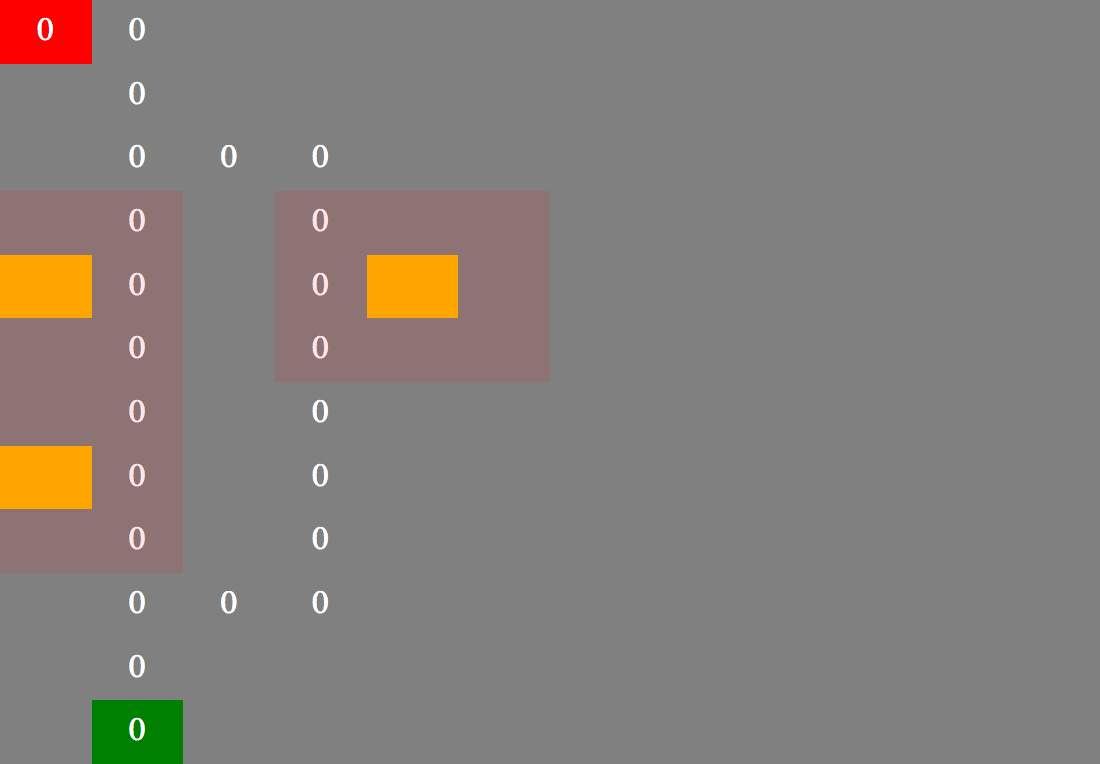
\includegraphics[width=1\linewidth]{images/map_shortlong}
  \caption{Simple short and long path Map, where the longer path is cheaper regarding deaths}
  \label{fig:mapshortlong}
\end{figure}


The second map we created is a mirrored one. The base layout contains a short and a long path. These are mirrored. One of the sides with the mirrored-layout contains towers, so it is always cheaper to use the correct side. It is displayed in Figure \ref{fig:mapsmirror}.

\begin{figure}[H]
  \centering
  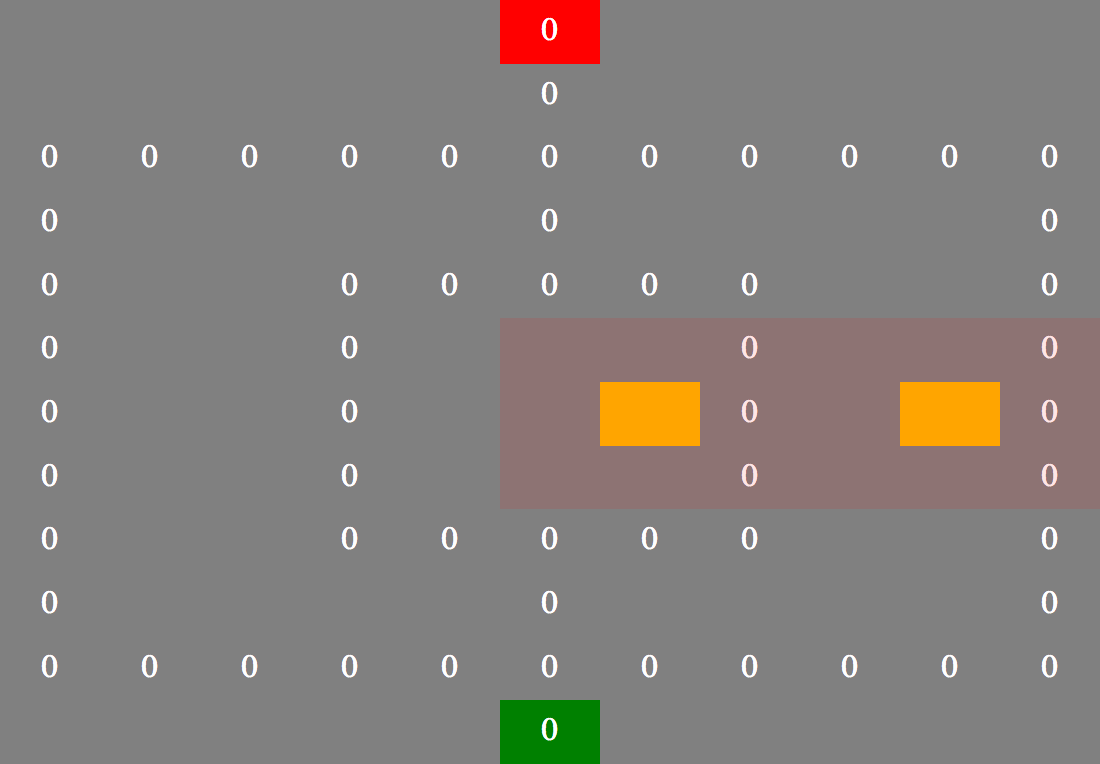
\includegraphics[width=1\linewidth]{images/map_mirror}
  \caption{Mirrored Map with two identically short paths, but one is better because it doesn't contain Towers.}
  \label{fig:mapsmirror}
\end{figure}


The third map we created came out of the idea to create a stress test for our continuous vapour strategy mentioned in Section \ref{sec:behaviour}. As deducible from Figure \ref{fig:mapsmaze} it is not directly obvious which path is the shortest one. But the longer path that leads through the top also contains a tower which makes it less attractive. The shortest two paths are following the bottom way to the target.

\begin{figure}[H]
  \centering
  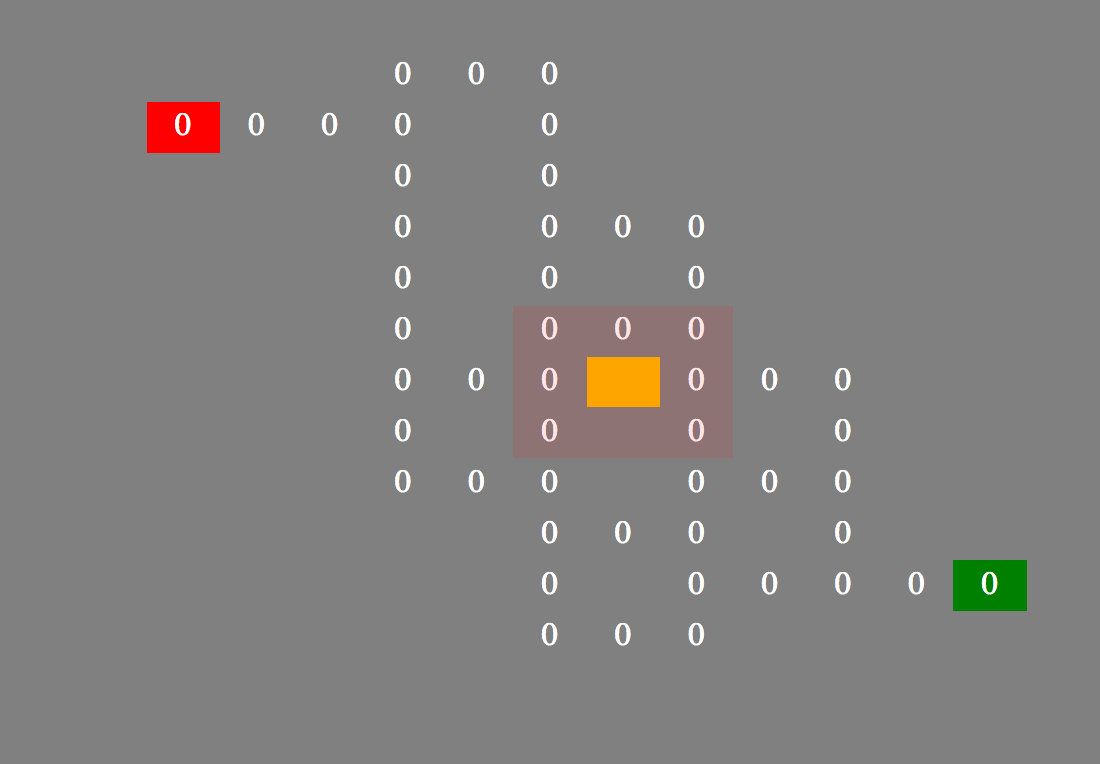
\includegraphics[width=1\linewidth]{images/map_maze}
  \caption{Maze Map created as a stress test for the continuous vapour strategy}
  \label{fig:mapsmaze}
\end{figure}
